\begin{figure}[H]
\centering
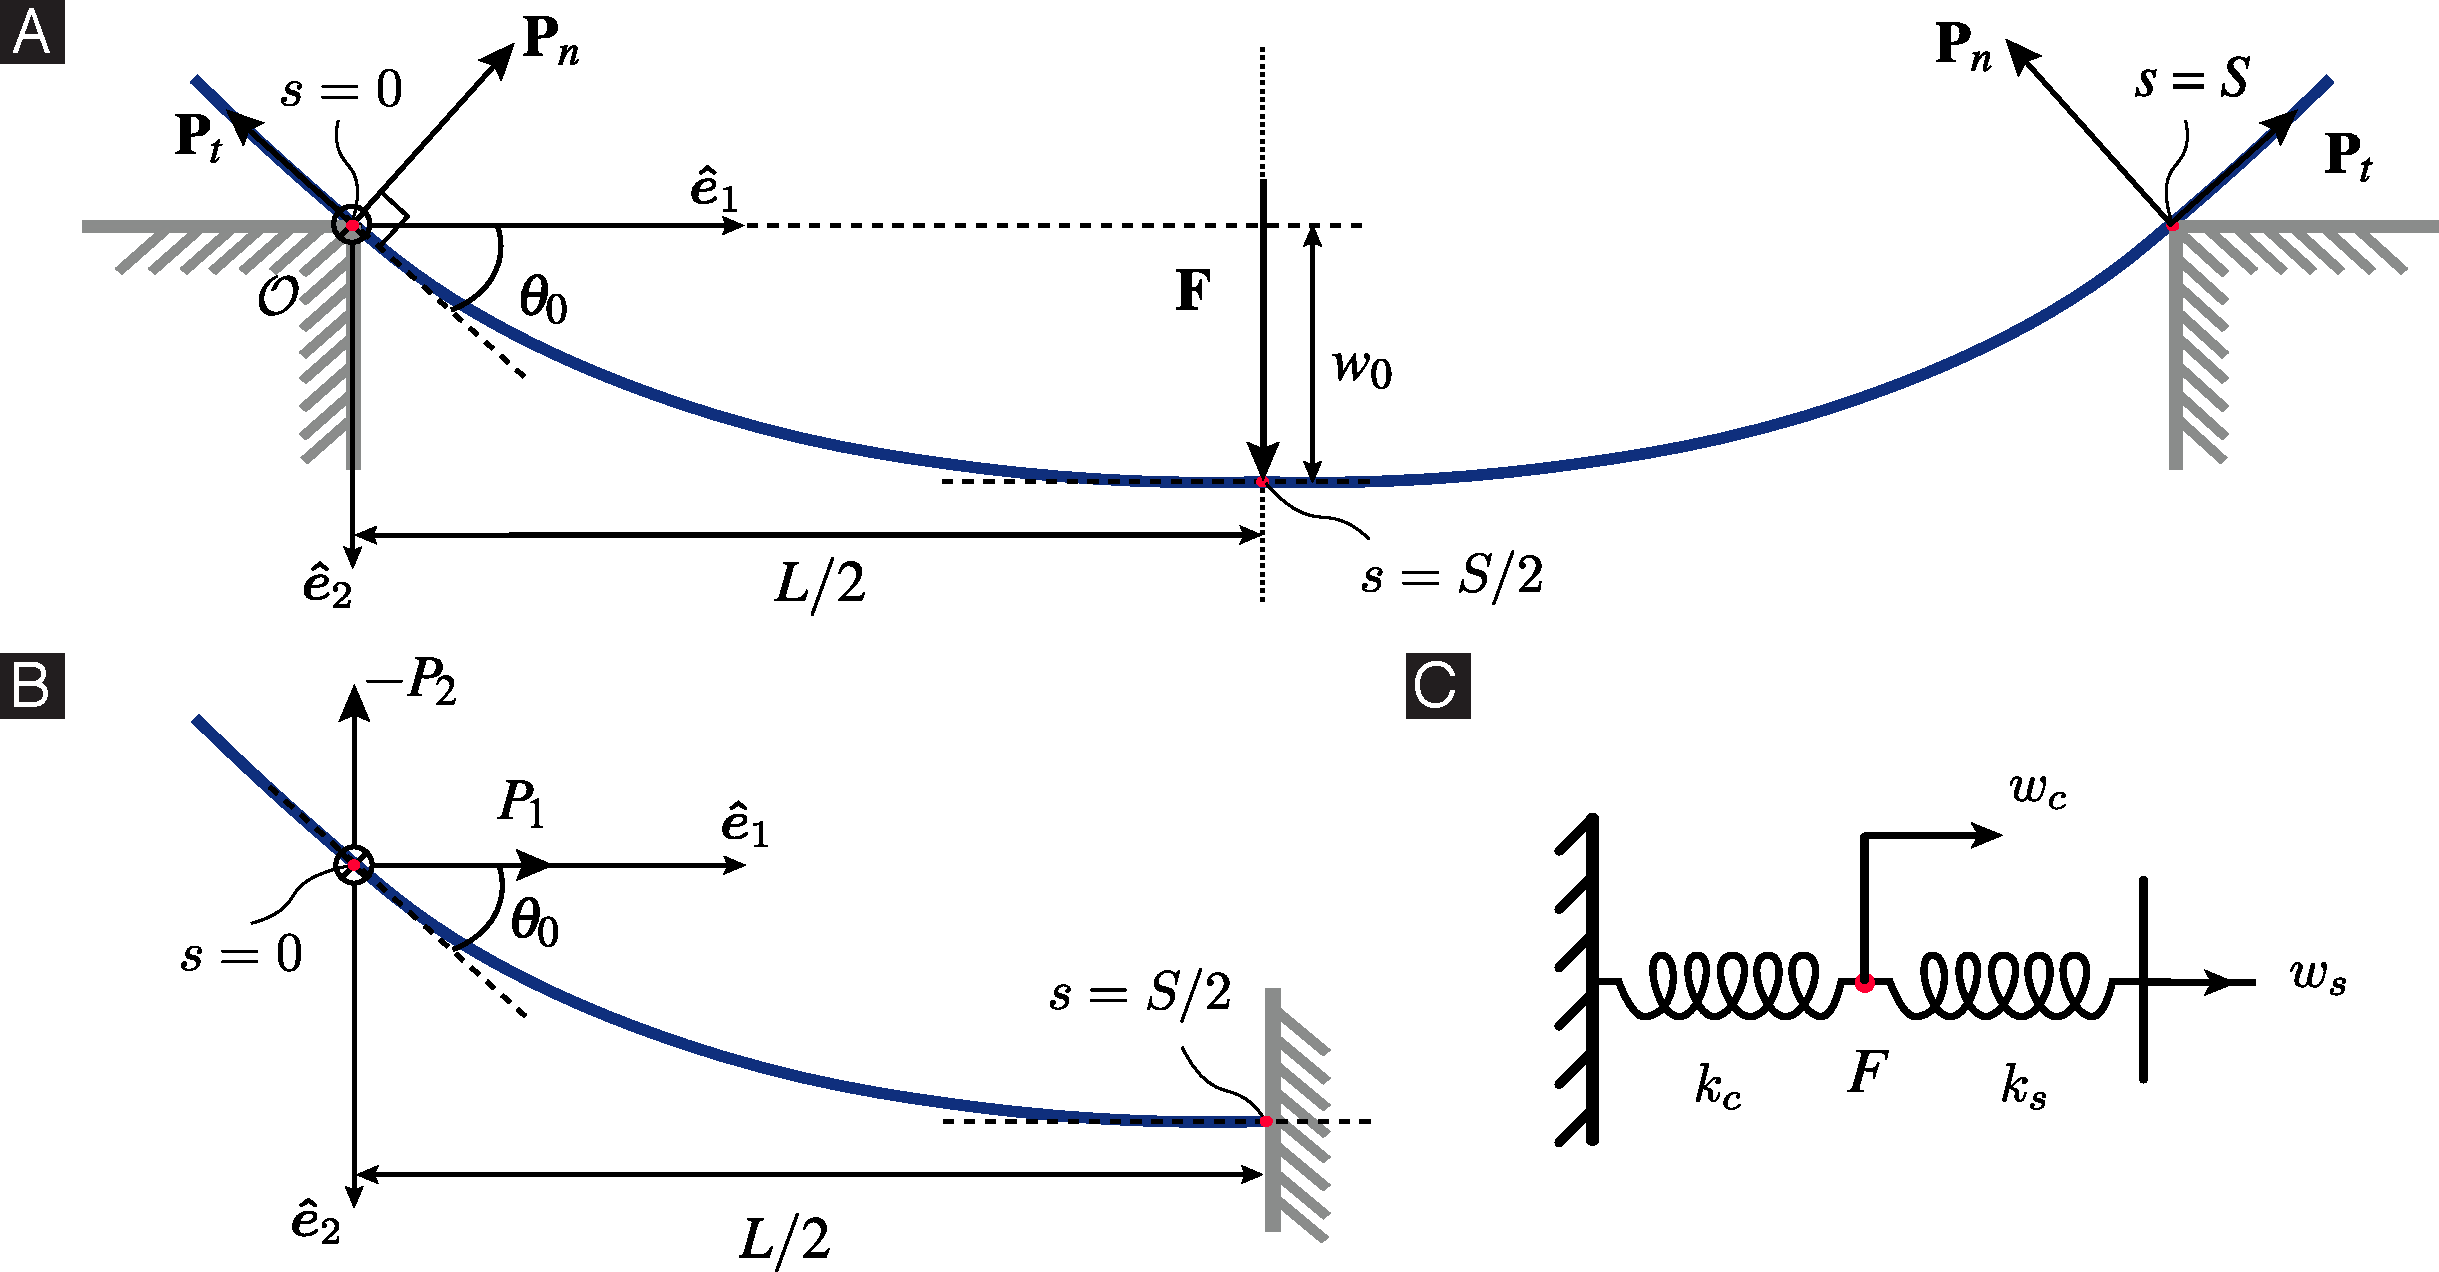
\includegraphics[width=0.9\textwidth]{Figures/BeamSchematic_V10.pdf}
\caption{Schematics of nonlinear bending-sliding model.
(\textsf{A}) A schematic of a simply-supported setup showing a beam (blue) suspended over the trench (grey) and applied force $\mathbf{F}$ located at mid span. The beam is experiencing normal reaction forces $\mathbf{P}_n$ and frictional forces $\mathbf{P}_t$ at $s = 0$ and $s = S$.
(\textsf{B}) A setup of cantilever beam with fixed end at $s = S/2$ and applied force $\mathbf{P} = P_1 \physf_1 + P_2 \physf_2 $ at $s = 0$.
(\textsf{C}) A schematic of a pair of springs in series. This is a mechanical simplication of the stiffness-controlled loading system.
}
\label{fig:BeamSchematic}
\end{figure}
